\documentclass[12pt,fleqn]{exam}
\usepackage{pifont}
\usepackage{dingbat}
\usepackage{amsmath,amssymb}
\usepackage{epsfig}
\usepackage[colorlinks=true,linkcolor=black,anchorcolor=black,citecolor=black,filecolor=black,menucolor=black,runcolor=black,urlcolor=black]{hyperref}
\usepackage[letterpaper, margin=0.75in]{geometry}
\usepackage{tikz}
\usepackage[super]{nth}
\usetikzlibrary{arrows}
\addpoints
\boxedpoints
\pointsinmargin
\pointname{pts}

\usepackage{pdfpages}
\usepackage[final]{microtype}
\usepackage[american]{babel}
\usepackage[T1]{fontenc}
\usepackage{fourier}
%\usepackage{eucal}

\usepackage{isomath}
\usepackage{upgreek,amsmath}
\usepackage{amssymb}
\usepackage{siunitx}

\newcommand{\dotprod}{\, {\scriptzcriptztyle
    \stackrel{\bullet}{{}}}\,}

\newcommand{\reals}{\mathbf{R}}
\newcommand{\lub}{\mathrm{lub}} 
\newcommand{\glb}{\mathrm{glb}} 
\newcommand{\complex}{\mathbf{C}}
\newcommand{\dom}{\mbox{dom}}
\newcommand{\range}{\mbox{range}}
\newcommand{\cover}{{\mathcal C}}
\newcommand{\integers}{\mathbf{Z}}
\newcommand{\degree}{\mathrm{degree}}
\newcommand{\vi}{\, \mathbf{i}}
\newcommand{\vj}{\, \mathbf{j}}
\newcommand{\vk}{\, \mathbf{k}}
\newcommand{\bi}{\, \mathbf{i}}
\newcommand{\bj}{\, \mathbf{j}}
\newcommand{\bk}{\, \mathbf{k}}
\newcommand{\dist}{\, \mathrm{dist}}
\DeclareMathOperator{\Arg}{\mathrm{Arg}}
\DeclareMathOperator{\Ln}{\mathrm{Ln}}
\newcommand{\imag}{\, \mathrm{i}}

\usepackage{tikz}
\usepackage{amsmath}
\usetikzlibrary{arrows}
\usepackage{xcolor}
\shadedsolutions
\definecolor{SolutionColor}{rgb}{0.95,0.95,0.95}

\usepackage{graphicx}
\newcommand\AM{{\sc am}}
\newcommand\PM{{\sc pm}}
     
%\usepackage{twemojis}
\newcommand{\quiz}{15}
\newcommand{\term}{Spring}
\newcommand{\due}{9:55 \AM}
\newcommand{\class}{MATH 102}
\begin{document}
\large
\vspace{0.1in}
\noindent\makebox[3.0truein][l]{\textbf{\class, \term \/ \the\year}}
\textbf{Name:} \hrulefill \\
\noindent \makebox[3.0truein][l]{\textbf{In class work \quiz}}
\textbf{Row and Seat}:\hrulefill\\
%\vspace{0.1in}

\small
\begin{flushleft}
  \emph{
 %   “Money buys everything except love, personality, freedom, immortality, silence, peace.”}
 %   \hfill \sc{Carl Sandburg}
  %  “Sometimes it's a little better to travel than to arrive.”}  \hfill {\sc  Robert M. Pirsig}
    “Self-education is, I firmly believe, the only kind of education there is.” 
    \hfill {\sc  Isaac Asimov }}
\end{flushleft}
 \large
%\noindent  In class work  \quiz\/  has questions 1 through  \numquestions \/ with a total of  \numpoints\/  points.   
% This assignment is due at the end of the class period (\due).
%This assignment is printed on \textbf{both} sides of the paper.
%\vspace{0.1in}


\begin{questions} 

\question Given that $F$ is a sequence and that $F_1 = 5, F_2 = 8$, and $F_3 = 42$.
Is $F$ an  \emph{arithmetic} sequence? Explain.

\begin{solution}[2.25in]

\end{solution}

\question Given that $Q$ is a sequence and that $Q_1 =2, Q_2 = 8$, and $Q_3 = 42$.
Is $Q$ an  \emph{geometric} sequence? Explain.

\begin{solution}[2.25in]

\end{solution}

\question Given that $G$ is an \emph{arithmetic} sequence and that $G_2 = 8$ and $G_4=9$, 
find a \emph{formula} for $G$.

\begin{solution}[2.25in]

\end{solution}
    
\question Given that $H$ is a \emph{geometric} sequence and that $H_2 = 8$ and $H_4=9$, 
find a \emph{formula} for $G$.

\begin{solution}[2.25in]

\end{solution}

\question Find the \emph{numerical value} of each sum
\begin{parts}
  \part $\displaystyle \sum_{k=1}^{46} 1$
  \begin{solution}[1.25in]

  \end{solution} 

  \part $\displaystyle \sum_{k=1}^{107} (2 k + 3)$
  \begin{solution}[1.25in]

  \end{solution} 
\end{parts}

\question Given that $W$ is an \emph{arithmetic sequence} and that $W_1=2$ and $W_2 = 3$,
find the numerical value of $\displaystyle \sum_{k=1}^{42} W_k$. 

\begin{solution}[2.25in]

\end{solution}
\question After graduation from UNK, you expect a first year salary of $\$70,000$
and you expect a raise of 4\% for each of the 42 years that you will work. Your salary
for your $\mbox{n}^{\mbox{th}}$ year of work $S_n$ is
\begin{equation*}
    S_n = 70000 \times 1.04^{n-1}
\end{equation*}

\begin{parts}
  \part Find the numerical value of $S_{42}$. This is your salary the year you retire.
  \begin{solution}[1.25in]

  \end{solution} 

  \part Over your career, your total earnings will be
  \begin{equation*}
       \sum_{k=1}^{42} 70000 \times 1.04^{k-1}.
  \end{equation*}
  Find the numerical value of your total earnings.
  You might like to use the fact that 
  $70000 \times 1.04^{k-1} = \frac{70000}{1.04}\times 1.04^{k}$
\end{parts}
\begin{solution}[1.25in]

\end{solution} 

\hfil
\newpage
\question The human population $P$ of Floyd, Virginia is an exponential function of the years $T$ after the year 2000.  Specifically,
the population in the years 2000 and 2010 are given in the table

\begin{figure*}[h]
\begin{center}
\begin{tabular}{|c|c|c|} \hline
  Year & $T$  & $P$ \\ \hline
  2000 & 0    & 432  \\
  2010 & 10   & 425  \\ \hline
  \end{tabular}.
  \caption{Human population of Floyd for the years 2000 and 2010.}
  \end{center}
\end{figure*}
\begin{parts}

\part [2] Find the exponential function that matches the given data.

\begin{solution}[2.0in] We just need to match to the general result in the QRS. That gives
   \begin{equation*}
       P = 341 \times \left(\frac{305}{341} \right)^{T/10}.
   \end{equation*}
   Converting this to the form $P = 341 \times \mathrm{e}^{-0.011157 \cdots \times T}$ \emph{isn't} required by the problem statement; so LIB.  And converting this to the form $P = 341 \times 0.98890\cdots^T$, \emph{isn't} required by the problem statement; so again LIB.
\end{solution}

\part [2] Using your exponential function from part `a,' when will the population of Floyd be 250?

\begin{solution}[3.0in] 
   We need to solve $280 = 341 \times \left(\frac{305}{341} \right)^{T/10}$ for $T$. Some (many) students will be more comfortable
   using decimal approximations to various quotients as they go. That's OK.
   \begin{align*}
   \left[280 = 341 \times \left(\frac{305}{341} \right)^{T/10} \right] &=
   \left[\frac{280}{341} = \left(\frac{305}{341} \right)^{T/10} \right] &\mbox{($\div$ 341)} \\
   &= \left[\log(\frac{280}{341}) = \log \left(\left(\frac{305}{341} \right)^{T/10} \right) \right] &\mbox{(log of left and right)} \\
   &= \left[\log \left (\frac{280}{341} \right) = \frac{T}{10} \log \left(\frac{305}{341}  \right) \right] &\mbox{(log property)} \\
   &= \left[T = 10 \times \frac{\log \left (\frac{280}{341} \right)}{\log \left(\frac{305}{341} \right)} \right], &\mbox{(divide)} \\
   &= \left[T \approx 17.7 \mbox{years} \right]. 
   \end{align*}

\end{solution}

\end{parts}

%\hfill
%\newpage


\question [2]  Find the solution to the linear equations
\begin{align*}
   5 x + 8 y &= 14, \\
   x -  y &= 3.
\end{align*}

\begin{solution}[3.0in] Let's use our matrix method. Ordering the unknowns as $x$  (first column) and $y$ (second column), 
   our system in matrix form is
   \begin{align*}
       \begin{bmatrix} 5 & 8 & 14 \\ 2 & -2 & 3 \end{bmatrix}
       \begin{bmatrix}  \\ 2 & R_2 \leftarrow 2 R_1 - 5 R_2 \end{bmatrix}
       &= \begin{bmatrix} 5 & 8 & 14 \\ 0 & 26 & 13 \end{bmatrix}
   \end{align*}
   The second equation is $26 y = 13$. So $y=\frac{1}{2}$. Pasting that into the 
   first equation gives $5 x + 4 = 14$. So $x =2$. 

   Should we check our work?  Sure. 
   \begin{equation*}    
      \left[5 x + 8y = 14\right] = \left[5 \times 2  + 8 \times \frac{1}{2} = 14\right] =
      \left[10 + 4 = 14\right] = \mbox{True!}      
   \end{equation*}
   And one more time
   \begin{equation*}    
      \left[2 x - 2 y = 3\right] = \left[2 \times 2  - 2 \times \frac{1}{2} = 3 \right] =
      \left[4 - 1 = 3\right] = \mbox{True!}      
   \end{equation*}
\end{solution}

\question [2] Find the solution to the linear equations
\begin{align*}
   x + y + z &= 6, \\
   y + z &= 10,\\
   y - z &= 20.
\end{align*}

\begin{solution} Ha! Let's be lazy and start at the bottom and work up! That gives $z=4$;
   so $y- 4 = 10$. So $y=14$. And finally $x + 14 + 4 = 14$. So $x = -4$.

\end{solution}

\question [2] Larry is saving his money to purchase a
1968 Fender Stratocaster Sunburst guitar.
To save for the guitar, he invests \$5,000 into a bank CD with an APY of 5.0\%. 
How long will Larry need to wait until he can purchase the Stratocaster that costs
\$7,700?

\begin{solution}[3.0in]
    We need to solve $12495 = 1000 \times 1.05^T$ for $T$. Since the unknown
    $T$ is an exponent, we'll use the \emph{logarithm trick}. Specifically,
    \begin{align*}
      \left[12495 = 10000 \times 1.05^T \right] &= \left[1.2495 = 1.05^T \right], &\mbox{(divide by 10000)} \\
                     &= \left[\log_{10}(1.2495) = \log_{10}(1.05^T) \right],  &\mbox{(logarithm trick)} \\
                     &= \left[\log_{10}(1.2495) = T \log_{10}(1.05) \right],  &\mbox{(logarithm property)} \\
                     &= \left[ T = \frac{\log_{10}(1.2495)}{\log_{10}(1.05)} \right],  &\mbox{(divide by $\log_{10}(1.05)$)} \\
                     &= \left[ T \approx 4.6 \mbox{ years} \right].  &\mbox{(arithmetic)}
    \end{align*}
Remember: $\log_{10}$ is \textbf{not} a multiplicative factor 
in the quotient $\displaystyle \frac{\log_{10}(1.2495)}{\log_{10}(1.05)}$. 
So do \textbf{not} cancel $\log_{10}$ in this expression.


\textbf{FYI:} The actor, storyteller, and musician Andy Griffith played a Martin D-18 guitar in the movie \emph{A face in the Crowd}\
that was painted black. He had the guitar restored and played it professionally
for many years. 

\quad Elvis owned two Martin D--18 guitars. His 1942 model recently sold for \$1.32 million. For this problem, I looked on eBay for the cost of
a Martin D--18 that wasn't owned by a celebrity. 
\end{solution}

\vfill
\newpage
\question [2] In April 2004, Ms Oro purchases one ounce of gold for \$647. 
Today (that is, twenty years later), Ms Oro sells her gold for \$1,995.
Find the APY for this investment.
\begin{solution}[3.0in]
We need to solve $1995 = 647 \times (1+r)^{20}$ for $r$. Since 
the unknown is in the base of an exponential, we use the \emph{root trick}.
Specifically,
\begin{align*}
    \left[1995 = 647 \times (1+r)^{20} \right] &= \left[\frac{1995}{647} = (1+r)^{20} \right], & \mbox{(divide by 647)}\\
               &= \left[\left(\frac{1995}{647}\right)^{1/20} = (1+r) \right], & \mbox{(root trick)} \\
               &= \left[r = \left(\frac{1995}{647}\right)^{1/20} - 1 \right], & \mbox{(subtract 1)}\\
               &= \left[ r \approx 5.79\% \right]. &\mbox{(arithmetic)}
\end{align*}
You might be more comfortable doing the arithmetic as you go, instead
of saving it up until the end. That's okay, but I think it makes it
more difficult to check the work, increases chances of miscopying
numbers, and it potentially decreases accuracy (by rounding intermediate results).
Try saving the arithmetic to the end--you might like it.

\textbf{FYI:} By investing in a stock index fund, Ms Oro would have
gotten a higher APY on her investment. For the cost of gold, I used 
actual historical data--I didn't just make it up.

And by the way: the Spanish word for gold is `oro.'


\end{solution}


\question To save for the purchase of a new 781 Porsche Boxster,
Morweena purchases a bond with a value of \$80,000 when it matures
in 20 years.

\begin{parts}

    \part [2] At the time of purchase, the 20 year APY is 5.0\%.
    Find the \emph{purchase price} of the bond.
    \begin{solution}[3.0in] We need to solve 
        $100000 = P \times 1.05^{30}$ for $P$. We have
        \begin{equation}
             P = \frac{100000}{1.05^{30}} \approx 23137.74.
        \end{equation}

    \end{solution}

    \part [2] After twenty years, Morweena decides to sell her bond and
    to use the proceeds to purchase an organic vanilla bean farm in Hawaii.
    At the time of sale, the 30 year APY is 4.0\%. Find the 
    sale price of the bond.
    \begin{solution}[3.0in] The future value of the bond is still
        \$100,000. Think of it this way: if you purchase the bond from 
        James and hold onto it until maturity, the Federal government
        will pay you \$100,000. So its future value is still \$100,000.        
        What has changed is both the time to maturity (was
        30 years, now is 25) and the APY (was 5.0\%, not is 4.0\%).
        We now need to solve $100000 = P \times 1.04^{25}$ for $P$. 
        We have
        \begin{equation}
             P = \frac{100000}{1.04^{25}} \approx 37511.68.
        \end{equation}

    \quad James made a pretty good investment. He purchased the bond for 
    \$23,137.74 and sold it five years later for \$37,511.68, making
    a profit of \$14, 373.94. The APY of this investment can be found by solving
    $37511.68 = 23137.74 \times (1+r)^5$ for $r$. The solution 
    is $r = 10.1\%$. And that's much greater than the APY of
    the bond.
    
    
    \emph{Falling interest rates make bonds more 
    valuable; rising interest rates make bonds less valuable.}


    \end{solution}




\end{parts}
\end{questions}
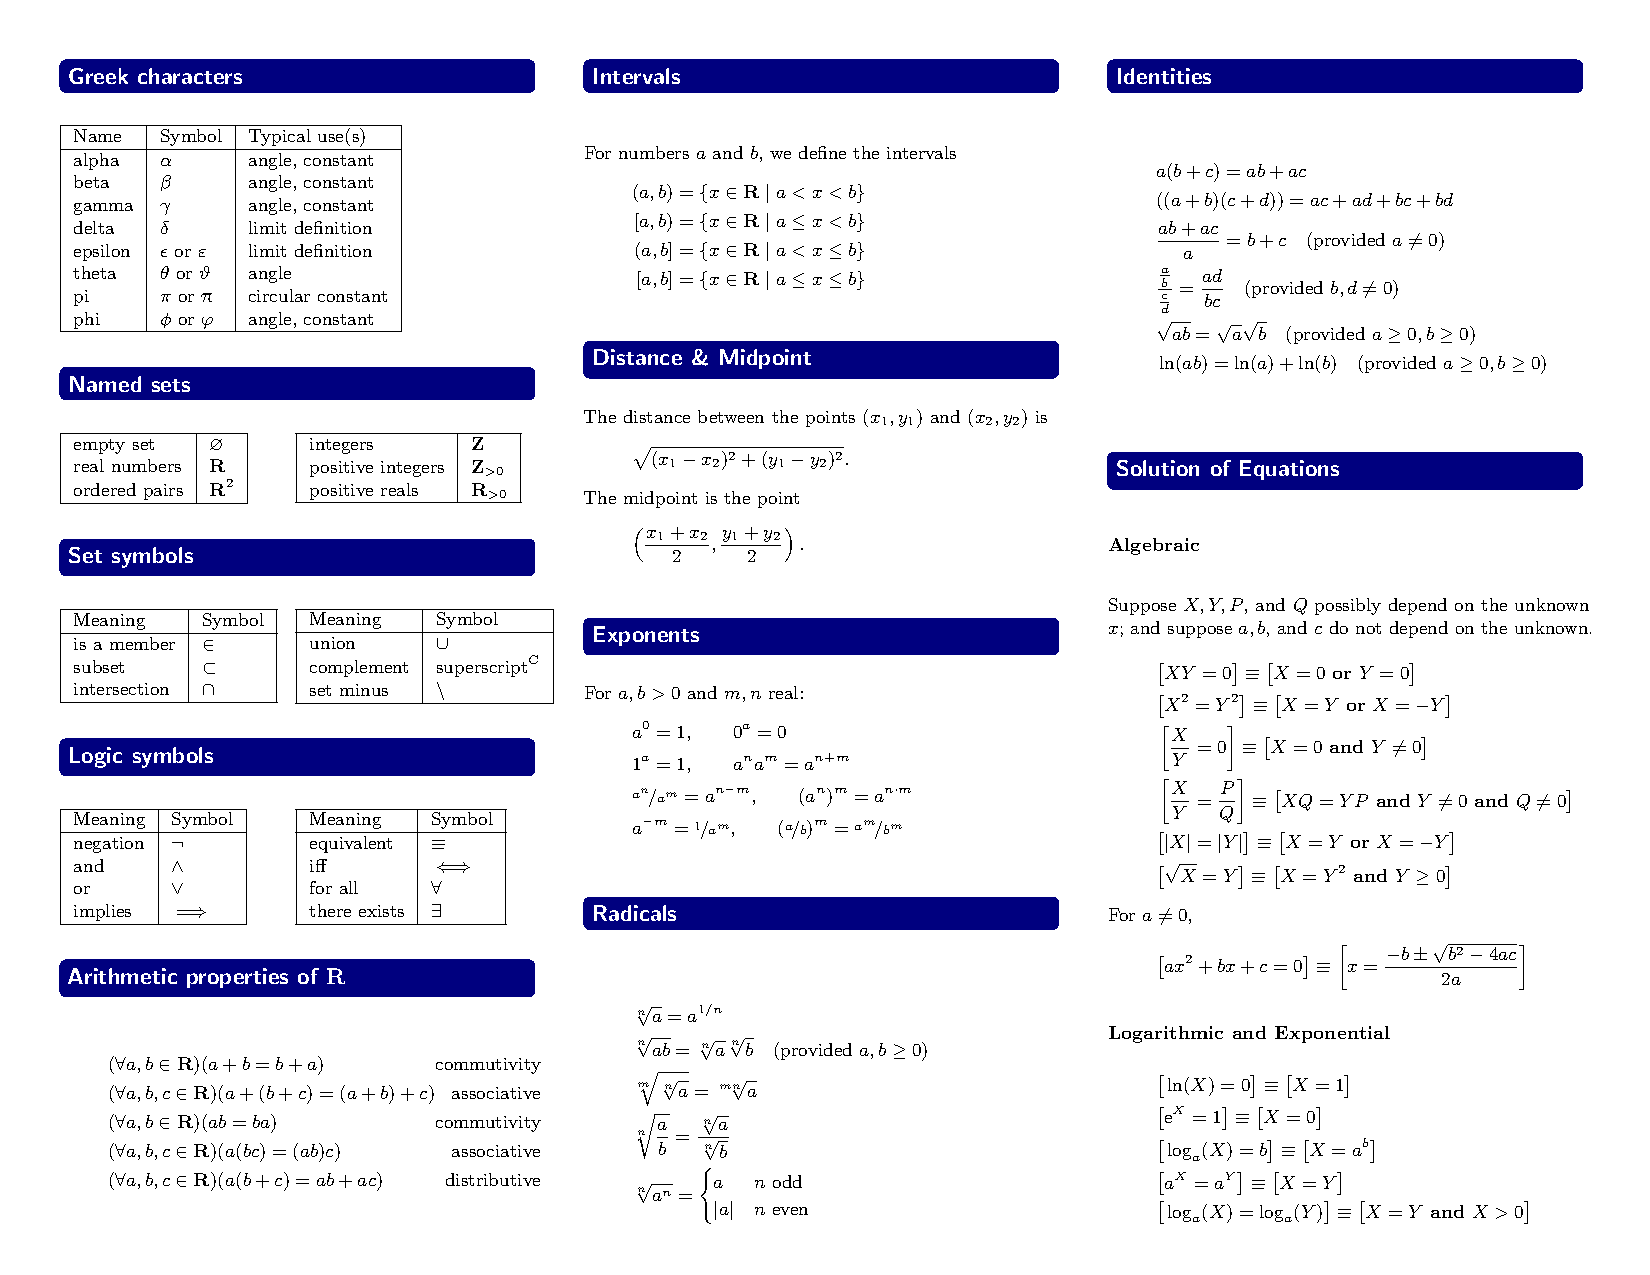
\includepdf[pages=-]{college-algebra-quick-reference}
\end{document}
